\documentclass{article}
\usepackage{a4wide}
\usepackage{graphicx}

\begin{document}


\begin{figure}[tb]
  \centering
  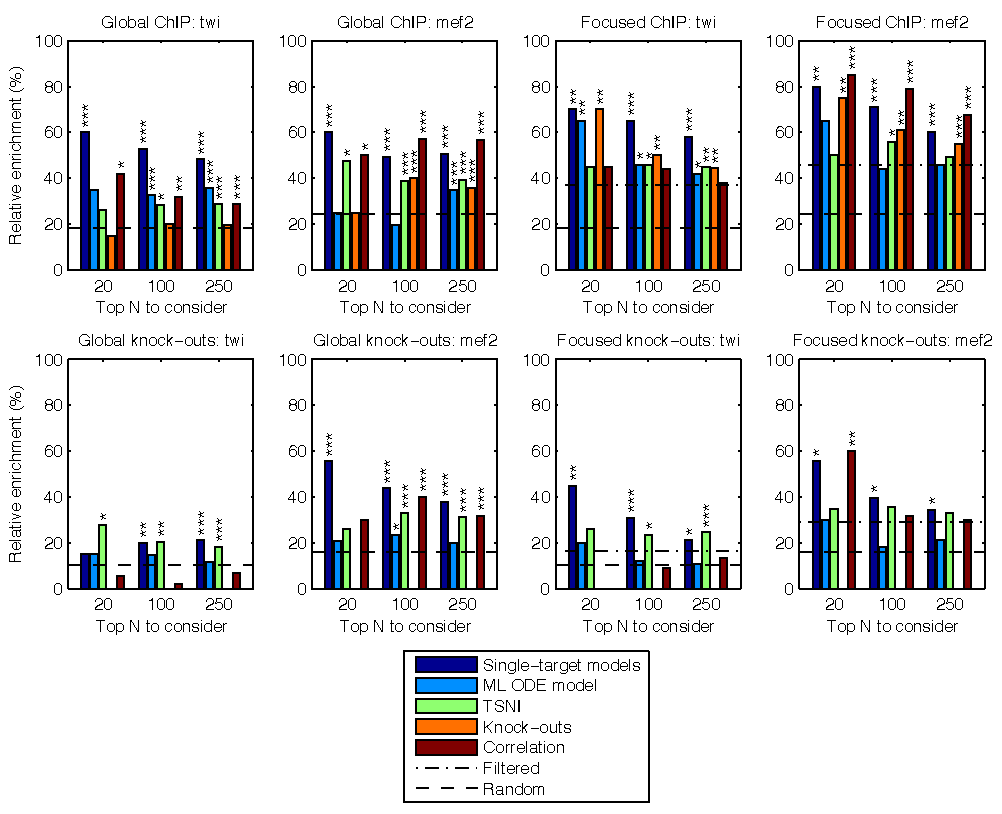
\includegraphics{Fig_S2}
  \caption{Global (left) and focused (right) evaluation results of different rankings 
    including a variant of the TSNI method of Della Gatta et al. (2008)
    using TF expression levels as a proxy
    for TF protein measurements showing the relative frequency of positive
    predictions among $N$ top-ranking targets, similar to Figures 3-4 in the
    main text.
    The dashed line
    denotes the frequency in the full population.
    The first row shows the frequency of targets with ChIP-chip
    binding within 2000 base pairs of the gene
    while the second row shows the frequency of
    predicted targets with significant differential
    expression in TF knock-outs.
    $p$-values of results significantly different from random are
    denoted by `***': $p <
    0.001$, `**': $p < 0.01$, `*': $p < 0.05$.
    Comparison to knock-out ranking is obviously omitted for knock-out
    validation. \label{fig:dros_global_evaluation}
  }
 % \label{fig:dros_global_evaluation}
\end{figure}

\end{document}
